\documentclass[12pt,twoside]{article}
%\documentclass[10pt,twoside,twocolumn]{article}
\usepackage[english]{babel}
\usepackage{times,subeqnarray}
\usepackage{url}
% following is for pdflatex vs. old(dvi) latex
\newif\myifpdf
\ifx\pdfoutput\undefined
%  \pdffalse           % we are not running PDFLaTeX
   \usepackage[dvips]{graphicx}
\else
   \pdfoutput=1        % we are running PDFLaTeX
%  \pdftrue
   \usepackage[pdftex]{graphicx}
\fi
\usepackage{apatitlepages}
% if you want to be more fully apa-style for submission, then use this
%\usepackage{setspace,psypub,ulem}
%\usepackage{setspace} % must come before psypub
%\usepackage{psypub}
%\usepackage{psydraft}
\usepackage{one-in-margins}  % use instead of psydraft for one-in-margs
\usepackage{scicite}
\usepackage{amsmath} % (JLR) Neede for "cases" in PredNet section
%\usepackage{apa}       % apa must come last
% using latex2e as standard, use the following for latex209
% \documentstyle [times,11pt,twoside,subeqnarray,psydraft,apa,epsf]{article}
\input netsym

% tell pdflatex to prefer .pdf files over .png files!!
\myifpdf
  \DeclareGraphicsExtensions{.pdf,.eps,.png,.jpg,.mps,.tif}
\fi

% use 0 for psypub format 
\parskip 2pt
% for double-spacing, determines spacing 
%\doublespacing
%\setstretch{1.7}

% rename figures as S1, etc
\setcounter{table}{0}
\renewcommand{\thetable}{S\arabic{table}}%
\setcounter{figure}{0}
\renewcommand{\thefigure}{S\arabic{figure}}%

\columnsep .25in   % 3/8 in column separation

\def\myheading{ Deep Predictive Learning Supplemental Materials}

% no twoside for pure apa style, use \markright with heading only
\pagestyle{myheadings}
\markboth{\hspace{.5in} \myheading \hfill}{\hfill O'Reilly, Russin, \& Rohrlich \hspace{.5in}}

\bibliographystyle{Science}

\title{ Supplementary Materials For:\\
Deep Predictive Learning as a Model of Human Learning } 

\author{Randall C. O'Reilly, Jacob L. Russin, and John Rohrlich\\
  Correspondence to: \texttt{oreilly@ucdavis.edu}\\}

\begin{document}

% sloppy is the way to go!
\sloppy
\raggedbottom
%\baselineskip20pt

\maketitle 

\noindent This PDF includes:
\begin{description}
\item Materials and Methods
\item Figures S1-S9
\item Table S1
\end{description}

\clearpage

\pagestyle{myheadings}

All of the materials described here, including the experimental study, the computational models, and the code to perform the representational similarity analysis, are all available on our github account at: \url{https://github.com/ccnlab/deep-obj-cat}  For the computational models in particular, the most complete understanding can only be had by directly examining the code for the models, as there are a number of details that are not efficiently captured in this suppplementary materials text.

\section{Representational Similarity Analysis Methods}

The different representations being compared here are:
\begin{description}
\item[Leabra:] The DeepLeabra (biological model) TE layer representations (specifically TEs = superficial -- results are very similar for deep as well).
\item[Bp:] The TEs layer representations from the backpropagation version of biological model, including {\em What, Where} and {\em What * Where} integration layers, trained with the V1p and V1hp (low and high resolution pulvinar) layers as final output layers, using the time $t$ target pattern from the $t-1$ input (i.e., as a predictive network).
\item[V1:] The gabor-filtered representation of the visual input to both of the above models, which was identical across them.
\item[PredNet:] Highest layer (4th Layer) of the PredNet architecture.

\item[Expt:] Similarity matrix constructed from human pairwise similarity judgments (see {\em Behavioral Experiment Methods}).
\end{description}

\begin{figure}
  \begin{tabular}{llll}
   \multicolumn{2}{c}{Centroid} & \multicolumn{2}{c}{Bp} \\
	% Centroid categories
	 \parbox[t]{1.4in}{\raggedright  	\baselineskip0pt
	\begin{enumerate}
	\item pyramid
	\begin{itemize}
	\item banana
	\item layercake
	\item trafficcone
	\item sailboat
	\item trex
	\end{itemize}
	\item vertical
	\begin{itemize}
	\item person
	\item guitar
	\item tablelamp
	\end{itemize}
	\item round
	\begin{itemize}
	\item doorknob
	\item donut
	\end{itemize}
	\end{enumerate}
	} & 
	 \parbox[t]{1.7in}{\raggedright 	\baselineskip0pt
	\begin{enumerate}
	\item[3.] round cont'd
	\begin{itemize}
	\item handgun
	\item chair
	\end{itemize}
	\item[4.] box
	\begin{itemize}
	\item slrcamera
	\item elephant
	\item piano
	\item fish
	\end{itemize}
	\item[5.] horiz
	\begin{itemize}
	\item car
	\item heavycannon
	\item stapler
	\item motorcycle
	\end{itemize}
	\end{enumerate}
	} &
	% Bp categories
	 \parbox[t]{1.4in}{\raggedright  	\baselineskip0pt
	\begin{enumerate}
	\item cat1
	\begin{itemize}
	\item banana
	\item layercake
	\item trafficcone
	\item sailboat
	\item trex
	\item person
	\item guitar
	\item tablelamp
	\item doorknob
	\item donut
	\end{itemize}
	\end{enumerate}
	} & 
	 \parbox[t]{1.7in}{\raggedright 	\baselineskip0pt
	\begin{enumerate}
	\item[1.] cat1 cont'd
	\begin{itemize}
	\item handgun
	\item chair
	\item slrcamera
	\item elephant
	\item piano
	\item fish
	\item car
	\end{itemize}
	\item[2.] cat2
	\begin{itemize}
	\item heavycannon
	\item stapler
	\item motorcycle
	\end{itemize}
	\end{enumerate}
	}\\
   \multicolumn{2}{c}{V1} \\
	% V1 categories
	 \parbox[t]{1.4in}{\raggedright  	\baselineskip0pt
	\begin{enumerate}
	\item cat1
	\begin{itemize}
	\item trafficcone
	\item sailboat
	\item person
	\item guitar
	\item tablelamp
	\item chair
	\end{itemize}
	\item cat2
	\begin{itemize}
	\item layercake
	\item trex
	\item doorknob
	\item donut
	\end{itemize}
	\end{enumerate}
	} & 
	 \parbox[t]{1.7in}{\raggedright 	\baselineskip0pt
	\begin{enumerate}
	\item[2.] cat2 cont'd
	\begin{itemize}
	\item handgun
	\item slrcamera
	\item elephant
	\item piano
	\item fish
	\item car
	\item heavycannon
	\item stapler
	\item motorcycle
	\end{itemize}
	\item[3.] cat3
	\begin{itemize}
	\item banana
	\end{itemize}
	\end{enumerate}
	}\\
	\end{tabular}
	\caption{Shape categories used for similarity matrix plots in main paper.  {\em Centroid} shape categories are near-best for both the Leabra model and the Expt results, and fit our visual intuitions about overall shape. {\em Bp} are reliably optimal for Bp model from all starting points.  {\em V1} are reliably optimal for V1 inputs, and also were best for the PredNet layer 3 representations.}
	\label{fig.cats}
\end{figure}

% (JLR) Should be layer *4* in PredNet, as you said earlier

An optimal category cluster can be defined as one that has high within-cluster similarity and low between-cluster similarity.  This can be operationalized by the {\em contrast} distance metric, based on a 1-correlation ({\em correlation distance}) measure, as the difference between the average within-cluster similarity and the average between-cluster similarity:
\begin{equation}
 cd = \langle 1-r_{in} \rangle - \langle 1-r_{out} \rangle 
\end{equation}
With distance-like 1-correlation values, this contrast distance should be minimized (it is typically negative), or equivalently the contrast on raw correlation values can be maximized (it is typically a positive number -- just the sign flip of distance value).  We refer to the positive numbers and maximization here as that is more natural.

Starting with an initial set of clusters, a permutation-based hill-climbing strategy was used to determine a local minimum in this measure: each item was tested in each of the other possible categories, and if that configuration reduced the overall average contrast distance metric across all items, then it was adopted and the process iterated until no such permutation improved the metric.  This algorithm can only decrease the number of clusters (by moving all items out of a given cluster), so different numbers of initial clusters can be used to search the overall space.

Figure~\ref{fig.cats} shows the resulting categories. The Bp model converged on the same cluster state from all starting configurations tested, varying from 5 to 2 initial categories.  This is the cluster set shown in Figure 4a of the main paper, and has an average contrast distance ({\em acd}) of 0.0838 (this is relatively low because the patterns were overall quite similar).  Likewise, the V1 patterns (which were the same across Leabra and Bp models) reliably converged on the same pattern (shown in Figure 4d), with {\em acd} = 0.2448.

For the PredNet layer3 representations, starting from the V1 categories was already optimal ({\em acd} = 0.0250 -- very low contrast overall), strongly indicating that it did not go beyond the structure present in the input, even though it did not use the V1 gabor filtering used in the Leabra and Bp models (i.e., this V1-level encoding well-captures the structure of the visual inputs in general).  The PredNet pixel and layer 0 representations both converged on essentially a single monolitic category with very low acd (0.0160).

% (JLR) Again - layer4, not 3

For the Leabra TE representations, we found a set of {\em centroid} shape categories that are near-best when considering both the Leabra model and the results from the human behavioral experiment (Expt).  Starting from these  categories, the permutation analysis converged on reducing the size of the vertical and round categories to one item each, over a sequence of 5 steps.  This is consistent with the observation from Figure 2a that there are three broader categories within which the 5 finer-grained categories are embedded (i.e., vertical and pyramid are overall similar to each other, as are round and box).  Nevertheless, our initial visual intuition about the broad shape categories, along with a bias against having single-item categories, reinforced the use of the finer-grained centroid selection.  The average contrast difference of our centroid selection is 0.5071, while the maximal result from the permutation was 0.5526, which is a relatively small proportional difference.

Furthermore, once we had collected the human experimental data ({\em Expt}), it was clear that it strongly coincided with our original shape intuitions, and with the finer-grained 5 category centroid structure.  Starting from the centroid categories, the maximal permutation made only 3 changes, moving trex (T-rex) and handgun into the horizontal category, and chair into the pyramid, going from a distance score of 0.3083 to 0.3225, which is a relatively small improvement.  However, using the maximal {\em Expt} clusters directly on the Leabra model gives a lower {\em acd} measure of 0.3745 (compared to 0.5071 for centroid), so the centroid categories represent a good middle-ground between experiment and the model, and this strong shared similarity structure with near-optimal cluster structures confirms that the model and people are encoding largely the same information.

In contrast, if we organize the experiment similarity matrix using the Bp categories, it produces a very poor average contrast distance measure of 0.0643 (compared to 0.3083 for the centroid categories), strongly suggesting that people's shape representations are not compatible with that simple structure.

\begin{figure}
  \centering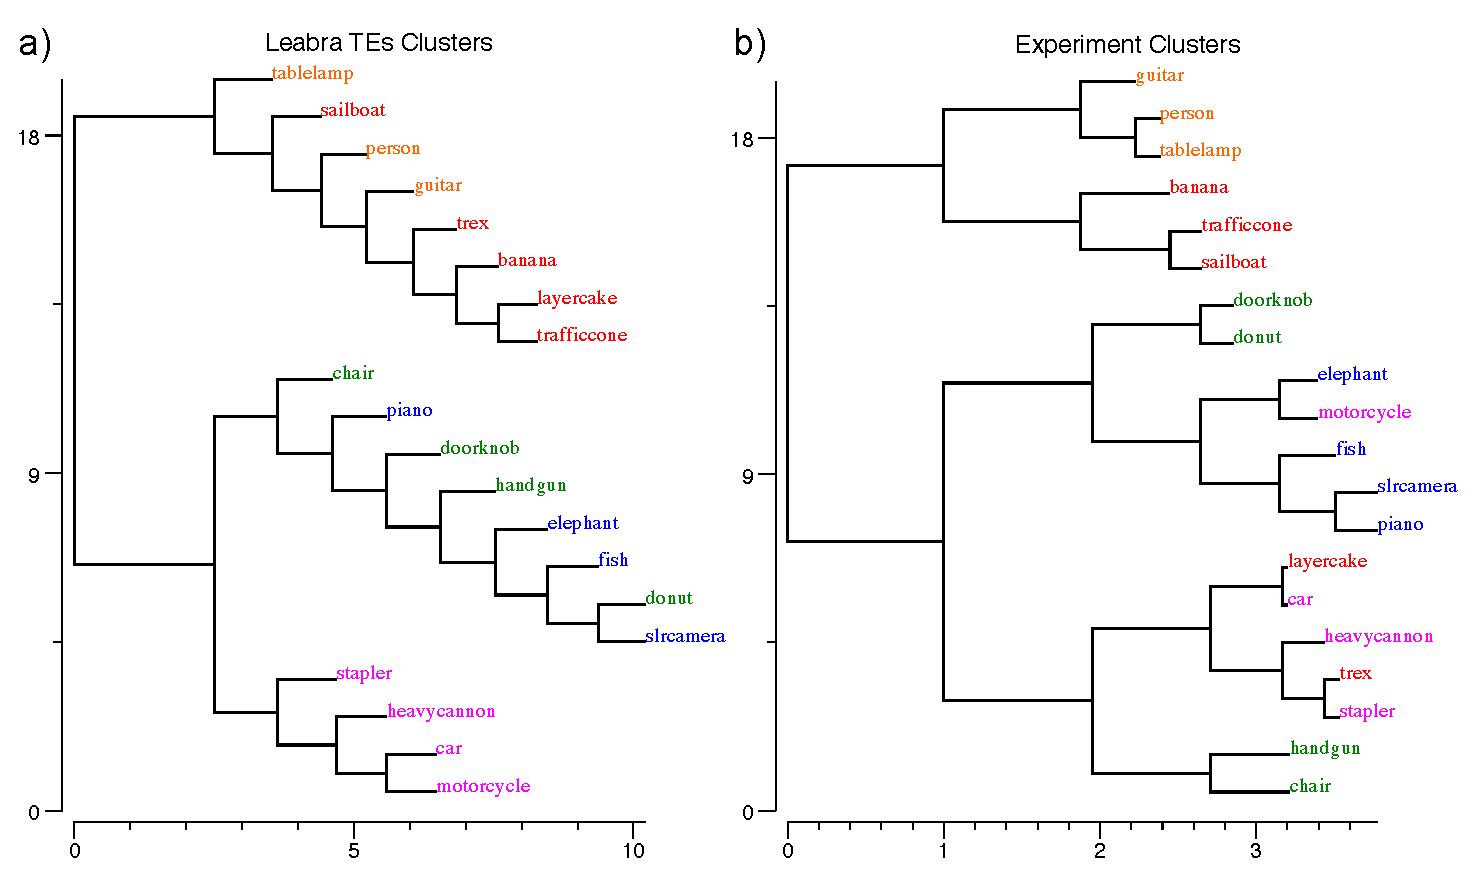
\includegraphics[width=6in]{figs/fig_deepleabra_wwi_clust_leabra_expt}
  \caption{ Agglomerative clustering on the Leabra and Expt representations, with the centroid categories color coded.  The most reliable information from this is the leaf-level groupings, as the rest of the structure is indeterminante and history dependent in reducing higher-dimensional structure down to a 2D plot.  Both cluster plots show a strong tendency to group leaf items together in the same centroid categories, with a few exceptions in each case.  Also, the Leabra plot nicely captures the broader 3-category structure evident in the similarity matrix plots, within which the 5 finer-grained centroid categories are organized.  Overall, this provides further confirmation that the model and the human subjects are organizing the shapes in largely the same way.}
  \label{fig.clust}
\end{figure}

Another approach to determining clusters from similarity matrices, {\em agglomerative clustering}, starts with all items as singletons, and iteratively combines the closest two into a new cluster.  The results for the Leabra and Expt similarity matrices are shown in Figure~\ref{fig.clust}, which has also color-coded the items in terms of their category status according to the centroid structure.  Due to a strong history dependency in the clustering process, and the indeterminacy of reducing a high-dimensional similarity structure down to two dimensions, structure beyond the leaf level is not very reliable (ties are also broken by a random number generator), but nevertheless you can clearly see that in both cases items from the same cluster are almost always together as leaves in the plots.  This then provides additional converging support for the idea that the model is learning the same kind of shape categories as people have.

% (JLR) Should add more detail about how RSA matrices are computed (e.g. averaging over samples, flattening all tensors into vectors, only using the representations from one of the frames of the video sequence)?

\section{Behavioral Experiment Methods}

\begin{figure}
  \centering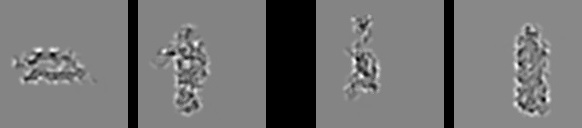
\includegraphics[width=4in]{figs/fig_deepleabra_wwi_expt1_trial_ex}
  \caption{Example stimulus from the behavioral experiment, using the V1 reconstruction of the actual input images presented to the model, to better capture the coarse-grained perception of the model.  Subjects were requested to choose which of the two pairs, Left or Right, was most similar in terms of {\em overall shape}.}
  \label{fig.expt}
\end{figure}

The behavioral experiment was conducted on Amazon.com's MTurk web platform under University of Colorado IRB approval (19-0176), using 30 participants each categorizing up to 800 image pairs as shown in Figure~\ref{fig.expt}, using the standard {\em simple image categorization} framework with a lightly customized script.  Objects were drawn from the 156 3D object set, but data was aggregated in terms of the 20 basic-level categories (car, stapler, etc) because we could not sample all 156 x 156 object pairs.  Thus, the resulting data was aggregated for each category pair in terms of the proportion of times when that pair was selected when presented.

The individual images were produced by reconstructing from the V1 transform that the computational model used in its high resolution V1 input layer, to give human participants as similar of an experience as possible to how the model ``saw'' the objects, and to reduce the influence of existing semantic knowledge which was entirely missing in our model (Figure~\ref{fig.expt}).

\section{Biological Model Methods}

This section provides more information about the {\em DeepLeabra} {\em What-Where Integration (WWI)} model.  The purpose of this information is to give more detailed insight into the model's function beyond the level provided in the main text, but with a model of this complexity, the only way to really understand it is to explore the model itself.  It is available for download at: \url{https://github.com/ccnlab/deep-obj-cat/sims/C++}  Furthermore, the best way to understand this model is to understand the framework in which it is implemented, which is explained in great detail, with many running simulations explaining specific elements of functionality, at \url{http://ccnbook.colorado.edu}

\subsection{Layer Sizes and Structure}

\begin{table}
  \centering
\begin{tabular}{llrrlll}
\hline
     &      & \multicolumn{2}{c}{{\bf Units}} & \multicolumn{2}{c}{{\bf Pools}} & \\
{\bf Area} & {\bf Name} & {\bf X} & {\bf Y} & {\bf X} & {\bf Y} & {\bf Receiving Projections} \\
\hline
V1 & V1s & 4 & 5 & 8 & 8 &  \\
   & V1p & 4 & 5 & 8 & 8 & V1s V2d V3d V4d TEOd  \\
V1h & V1hs & 4 & 5 & 16 & 16 &  \\
   & V1hp & 4 & 5 & 16 & 16 & V1s V2d V3d V4d TEOd  \\
Eyes & EyePos & 21 & 21 & & &  \\
     & SaccadePlan & 11 & 11 & & &  \\
     & Saccade & 11 & 11 & & &  \\
Obj & ObjVel & 11 & 11 & & & \\
V2 & V2s & 10 & 10 & 8 & 8 & V1s LIPs V3s V4s TEOd V1p V1hp \\
   & V2d & 10 & 10 & 8 & 8 & {\bf V2s} V1p V1hp LIPd LIPp V3d V4d V3s TEOs \\
LIP & MtPos& 1 & 1 & 8 & 8 & V1s \\
    & LIPs & 4 & 4 & 8 & 8 & MtPos ObjVel SaccadePlan EyePos LIPp \\
    & LIPd & 4 & 4 & 8 & 8 & {\bf LIPs} LIPp ObjVel Saccade EyePos \\
    & LIPp & 1 & 1 & 8 & 8 & {\bf MtPos} V1s LIPd \\
V3 & V3s & 10 & 10 & 4 & 4 & V2s V4s TEOs DPs LIPs V1p V1hp DPp TEOd \\
   & V3d & 10 & 10 & 4 & 4 & {\bf V3s} V1p V1hp DPp LIPd DPd V4d V4s DPs TEOs \\
   & V3p & 10 & 10 & 4 & 4 & {\bf V3s} V2d DPd TEOd \\
DP & DPs & 10 & 10 & & & V2s V3s TEOs V1p V1hp V3p TEOp \\
   & DPd & 10 & 10 & & & {\bf DPs} V1p V1hp DPp TEOd \\
   & DPp & 10 & 10 & & & {\bf DPs} V2d V3d DPd TEOd \\
V4 & V4s & 10 & 10 & 4 & 4 & V2s TEOs V1p V1hp \\
   & V4d & 10 & 10 & 4 & 4 & {\bf V4s} V1p V1hp V4p TEOd TEOs \\
   & V4p & 10 & 10 & 4 & 4 & {\bf V4s} V2d V3d V4d TEOd \\
TEO & TEOs & 10 & 10 & 4 & 4 & V4s V1p V1hp TEs\\
   & TEOd & 10 & 10 & 4 & 4 & {\bf TEOs TEOd} V1p V1hp V4p TEOp TEp TEd \\
   & TEOp & 10 & 10 & 4 & 4 & {\bf TEOs} V3d V4d TEOd TEd \\
TE & TEs & 10 & 10 & 4 & 4 & TEOs V1p V1hp \\
   & TEd & 10 & 10 & 4 & 4 & {\bf TEs TEd} V1p V1hp V4p TEOp TEp TEOd \\
   & TEp & 10 & 10 & 4 & 4 & {\bf TEs} V3d V4d TEOd \\
\hline
\end{tabular}
\caption{Layer sizes, showing numbers of units in one pool (or entire layer if Pool is missing), and the number of Pools of such units, along X,Y axes.  Each area has three associated layers: {\em s} = superficial layer, {\em d} = deep layer (context updated by 51B neurons in same area, shown in bold), {\em p} = pulvinar layer (driven by 5IB neurons from associated area, shown in bold).}
\label{tab.layer_sizes}
\end{table}

Figure~1 in the main text shows the general configuration of the model, and Table~\ref{tab.layer_sizes} shows the specific sizes of each of the layers, and where they receive inputs from. 

All the activation and general learning parameters in the model are at their standard Leabra defaults.

\subsection{Projections}

\begin{figure}
  \centering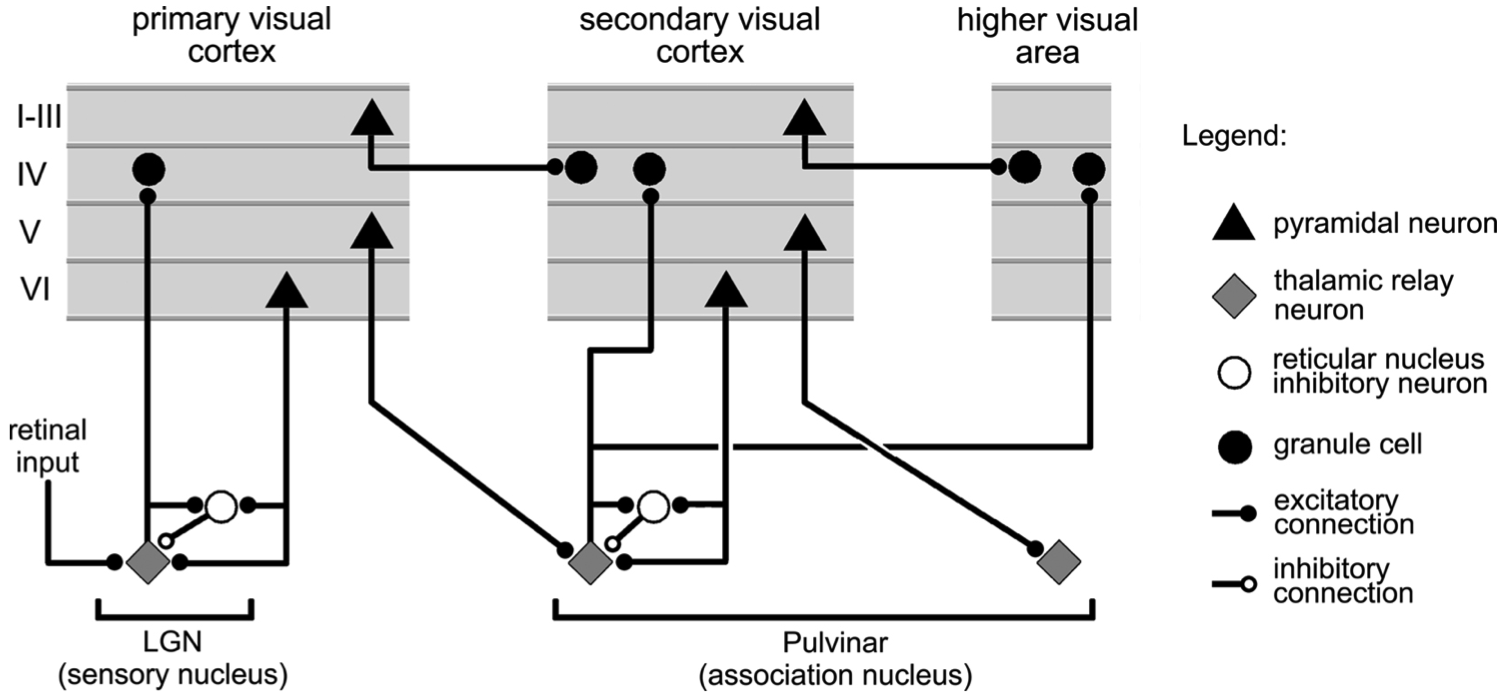
\includegraphics[width=4in]{figs/fig_sherman_guillery_summary}
  \caption{Summary figure from Sherman \& Guillery (2006) showing the strong feedforward driver projection eminating from layer 5IB cells in lower layers (e.g., V1), and the much more numerous feedback ``modulatory'' projection from layer 6CT cells.  We interpret these same connections as providing a prediction (6CT) vs. outcome (5IB) activity pattern over the pulvinar.  Note that much of the bursting dynamics discussed by these authors is not found in awake behaving animals, where pulvinar neurons exhibit sustained activity over the course of visual inputs similar to what is observed in corresponding visual areas (Robinson, 1993).}
  \label{fig.sandg}
\end{figure}

\begin{figure}
  \centering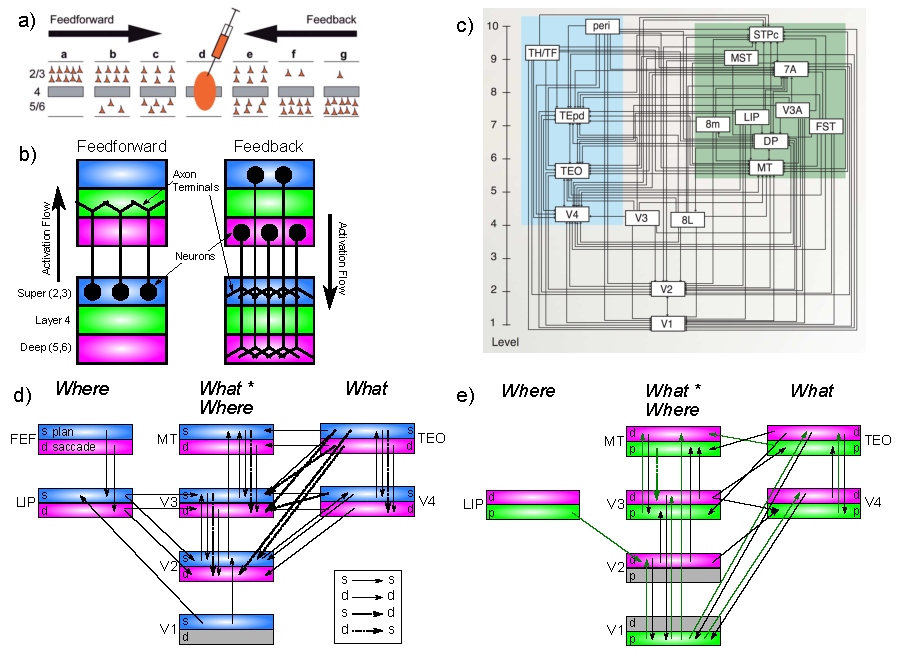
\includegraphics[width=5in]{figs/fig_deepleabra_wwi_cons_all}
  \caption{Principles of connectivity in DeepLeabra.  {\bf a)} Markov et al (2014) data showing density of {\em retrograde} labeling from a given injection in a middle-level area (d): most feedforward projections originate from superficial layers of lower areas (a,b,c) and deep layers predominantly contribute to feedback (and more strongly for longer-range feedback).  {\bf b)} Summary diagram showing most feedforward connections originating in superficial layers of lower area, and terminating in layer 4 of higher area, while feedback connections can originate in either superficial or deep layers, and in both cases terminate in both superficial and deep layers of the lower area (adapted from Felleman \& Van Essen, 1991). {\bf c)} Anatomical hierarchy as determined by percentage of superficial layer source labeling (SLN) by Markov et al (2014) --- the hierarchical levels are well matched for our model, but we functionally divide the dorsal pathway (shown in green background) into the two separable components of a {\em Where} and a {\em What * Where} integration pathway.  {\bf d)} Superficial and deep-layer connectivity in the model.  Note the repeating motif between hierarchically-adjacent areas, with bidirectional connectivity between superficial layers, and feedback into deep layers from both higher-level superficial and deep layers, according to canonical pattern shown in panels a and b.  Special patterns of connectivity from TEO to V3 and V2, involving crossed super-to-deep and deep-to-super pathways, provide top-down support for predictions based on high-level object representations. {\bf e)} Connectivity for deep layers and pulvinar in the model, which generally mirror the corticocortical pathways (in d).  Each pulvinar layer (p) receives 5IB driving inputs from the labeled layer (e.g., V1p receives 5IB drivers from V1).  In reality these neurons are more distributed throughout the pulvinar, but it is computationally convenient to organize them together as shown.  Deep layers (d) provide predictive input into pulvinar, and pulvinar projections send error signals (via temporal differences between predictions and actual state) to {\em both} deep and superficial layers of given areas (only d shown).  Most areas send deep-layer prediction inputs into the main V1p prediction layer, and receive reciprocal error signals therefrom.  The strongest constraint we found was that pulvinar outputs (colored green) must generally project only to higher areas, not to lower areas, with the exceptions of DPp $\rightarrow$ V3 and LIPp $\rightarrow$ V2.  V2p was omitted because it is largely redundant with V1p in this simple model.}
  \label{fig.model_cons}
\end{figure}

The general principles and patterns of connectivity are shown in Figures~\ref{fig.sandg} and \ref{fig.model_cons}.

Detailing each of the specific parameters associated with the different projections shown in Table~\ref{tab.layer_sizes} would take too much space --- those interested in this level of detail should download the model from the link shown above.  There are topographic projections between many of the lower-level retinotopically-mapped layers, consistent with our earlier vision models %\cite{OReillyWyatteHerdEtAl13}
{\em (31)}.  For example the 8x8 unit groups in V2 are reduced down to the 4x4 groups in V3 via a 4x4 unit-group topographic projection, where neighboring units have half-overlapping receptive fields (i.e., the field moves over 2 unit groups in V2 for every 1 unit group in V3), and the full space is uniformly tiled by using a wrap-around effect at the edges.  Similar patterns of connectivity are used in current deep convolutional neural networks.  However, we do not share weights across units as in a true convolutional network.

The projections from ObjVel (object velocity) and SaccadePlan layers to LIPs, LIPd were initialized with a topographic sigmoidal pattern that moved as a function of the position of the unit group, by a factor of .5, while the projections from EyePos were initialized with a gaussian pattern.  These patterns multiplied uniformly distributed random weights in the .25 to .75 range, with the lowest values in the topographic pattern having a multiplier of .6, while the highest had a multiplier of 1 (i.e., a fairly subtle effect).  This produced faster convergence of the LIP layer when doing {\em Where} pathway pre-training compared to purely random initial weights.  In addition to exploring different patterns of overall connectivity, we also explored differences in the relative strengths of receiving projections, which can be set with a \texttt{wt\_scale.rel} parameter in the simulator.  All feedforward pathways have a default strength of 1.  For the feedback projections, which are typically weaker (consistent with the biology), we explored a discrete range of strengths, typically .5, .2, .1, and .05.  The strongest top-down projections were into V2s from LIP and V3, while most others were .2 or .1.  Likewise projections from the pulvinar were weaker, typically .1.  These differences in strength sometimes had large effects on performance during the initial bootstrapping of the overall model structure, but in the final model they are typically not very consequential for any individual projection.

\subsection{Training Parameters}

\begin{figure}
  \centering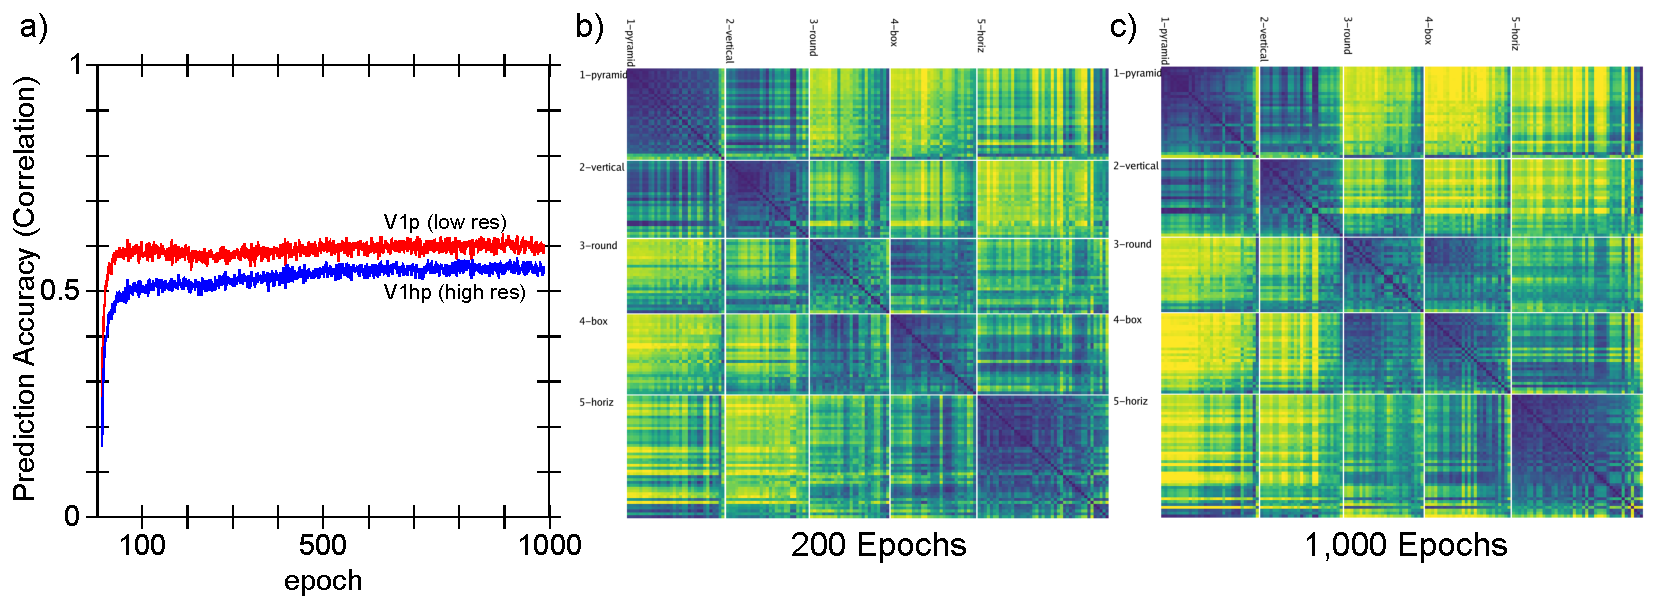
\includegraphics[width=5.5in]{figs/fig_deepleabra_wwi_emer_lrn_v1p_simat}
  \caption{{\bf a)} Predictive learning curve for DeepLeabra, showing the correlation between prediction and actual over the two different V1 layers.  Initial learning is quite rapid, followed by a slower but progressive learning process that reflects development of the IT representations (e.g., manipulations that interfere with those areas selectively impair this part of the learning curve).  Overall prediction accuracy remains far from perfect, as shown in Figure~1c in main text, and significantly worse than the backpropagtion-based models.  This is a typical finding from Leabra models which are significantly more constrained as a result of bidirectional attractor dynamics, Hebbian learning, and inhibitory competition -- i.e., the very things that are likely important for forming abstract catgorical representations. {\bf b)} Similarity matrix over TEs layer at 200 epochs, which has less contrast and definition compared to the 1,000 epoch result ({\bf c} also shown in Figure~2a in main text).}
  \label{fig.lrn}
\end{figure}

Training typically consisted of 512 alpha trials per epoch (51.2 seconds of real time equivalent), for 1,000 such epochs. Each trial was generated from a virtual reality environment in the emergent simulator, that rendered first-person views with moving eye position onto the object tumbling through space with fixed motion and rotation parameters over the sequence of 8 frames (see Figure~1c in main text for representative example).  Because the start of each sequence of 8 frames is unpredictable, we turned off learning for that trial, which improves learning overall.  We have recently developed an automatic such mechanism based on the running-average (and running variance) of the prediction error, where we turn off learning whenever the current prediction error z-normalized by these running average values is below 1.5 standard deviations, which works well, and will be incorporated into future models.  Biologically, this could correspond to a connection between pulvinar and neuromodulatory areas that could regulate the effective learning rate in this way.

Figure~\ref{fig.lrn}a shows the learning trajectory of the model, indicating that it learns quite rapidly.  This rapid initial learning is likely facilitated by the extensive use of shortcut connections convering from all over the simulated visual system onto the V1 pulvinar layers, and direct projections back from these pulvinar layers.  Thus, error signals are directly communicated and can drive learning quickly and efficiently.  However, there are also extensive indirect, bidirectional connections among the superficial layers, which can drive indirect error backpropagation learning as well.

\subsection{Testing Parameters}

To be able to monitor similarity metrics as the model trained, we used a running-average integration of neural activity across trials to accumulate the patterns used for the RSA analysis described above.  Specifically, for each object, and each frame, the current activation pattern across each layer was recorded and averaged unit-by-unit with a time constant of $\tau = 10$. Critically, by integrating separately for each frame, this running-average computation did not introduce any bias for temporally-adjacent frames to be more similar.  Nevertheless, when we computed the frame-to-frame similarities for TE, they were quite high (.901 correlation on average across all objects).

\subsection{Model Algorithms}

The biologically-based model was implemented using the Leabra framework, which is described in detail in previous publications %\cite{OReillyMunakataFrankEtAl12,OReillyMunakata00,OReilly98,OReilly96}
{\em (6,12,13,34)}, and summarized here.  There are two main implementations of Leabra, one in the {\em C++ emergent} software, and a new one using  Go and Python language at: \url{https://github.com/emer/leabra}.  There are also other simpler implementations in Python and MATLAB, see \url{https://grey.colorado.edu/emergent/index.php/Leabra}.   Both of the preceeding links contain a full detailed description of the algorithm.  These same equations and standard parameters have been used to simulate over 40 different models in % \cite{OReillyMunakataFrankEtAl12,OReillyMunakata00}
{\em (12,13)}, and a number of other research models.  Thus, the model can be viewed as an instantiation of a systematic modeling framework using standardized mechanisms, instead of constructing new mechanisms for each model.  Here, we only detail properties of the predictive learning algorithm that go beyond the basic Leabra model.

\subsubsection{Deep Context}

At the end of every plus phase, a new deep-layer context net input is computed from the dot product of the context weights times the sending activations, just as in the standard net input:
\begin{equation}
 \eta = \langle x_i \wij \rangle = \oneo{n} \sum_i x_i \wij
 \label{eq.net_in_ti}
\end{equation}
This net input is then added in with the standard net input at each cycle of processing.

% (JLR) I'm pretty confused here - what are these context layers for?
% (JLR) The math is also confusing/unclear. Would be helpful to have a sentence afterward explaining what each term is, like "..., where x_i is blah, w_ij is blah"
% (JLR) Also I think the dot product is written incorrectly. If w_j is its own vector (what does j index?), where w_ij is each element in that vector, then the "i" index should be removed from the x_i and w_ij in the inner product defintion: \eta = \langle x, w_j \rangle = \oneo{n} \sum_i x_i \wij
% (JLR) Also, dot product technically refers to the sum, not the average, i.e. without the 1/n?

The relative strength of these context layer inputs was set progressively larger for higher layers in the network, with a maximum of 4 in V4, TEO, and TE.  In addition, TEO and TE received {\em self} context projections which provide an extended window of temporal context into the prior 200 msec interval.  These self projections were connected only within the narrower Pool level of units, enabling these neurons to develop mutually-excitatory loops to sustain activations over the multiple trials when the same object was present.  We hypothesize that these modifications correspond to biological adaptations in IT cortex that likewise support greater sustained activation of object-level representations.

Learning of the context weights occurs as normal, but using the sending activation states from the {\em prior} time step's activation.

\subsubsection{Computational and Biological Details of SRN-like Functionality}

% (JLR) "SRN" = "simple recurrent network" is not introduced anywhere

Predictive auto-encoder learning has been explored in various frameworks, but the most relevant to our model comes from the application of the SRN to a range of predictive learning domains %\cite{Elman90,ElmanBatesKarmiloff-SmithEtAl96}
{\em (10,11)}.  One of the most powerful features of the SRN is that it enables error-driven learning, instead of arbitrary parameter settings, to determine how prior information is integrated with new information.  Thus, SRNs can learn to hold onto some important information for a relatively long interval, while rapidly updating other information that is only relevant for a shorter duration.  This same flexibility is present in our DeepLeabra model.  Furthermore, because this temporal context information is hypothesized to be present in the deep layers throughout the entire neocortex (in every microcolumn of tissue), the DeepLeabra model provides a more pervasive and interconnected form of temporal integration compared to the SRN, which typically just has a single temporal context layer associated with the internal ``hidden'' layer of processing units.

An extensive computational analysis of what makes the SRN work as well as it does, and explorations of a range of possible alternative frameworks, has led us to an important general principle: {\em subsequent outcomes determine what is relevant from the past}.  At some level, this may seem obvious, but it has significant implications for predictive learning mechanisms based on temporal context.  It means that the information encoded in a temporal context representation cannot be learned at the time when that information is presently active.  Instead, the relevant contextual information is learned on the basis of what happens next.  This explains the peculiar power of the otherwise strange property of the SRN: the temporal context information is preserved as a {\em direct copy} of the state of the hidden layer units on the previous time step (Figure~\ref{fig.srn_vs_ti}), and then learned synaptic weights integrate that copied context information into the next hidden state (which is then copied to the context again, and so on).  This enables the error-driven learning taking place in the {\em current} time step to determine how context information from the {\em previous} time step is integrated.  And the simple direct copy operation eschews any attempt to shape this temporal context itself, instead relying on the learning pressure that shapes the hidden layer representations to also shape the context representations.  In other words, this copy operation is essential, because there is no other viable source of learning signals to shape the nature of the context representation itself (because these learning signals require future outcomes, which are by definition only available later).

\begin{figure}
  \centering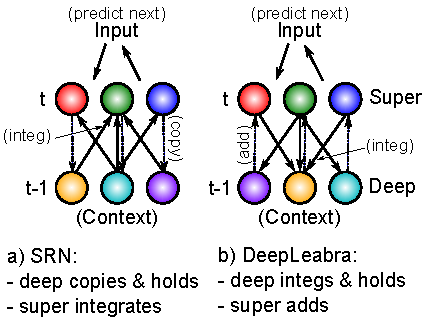
\includegraphics[width=3in]{figs/fig_srn_ti_compute}
  \caption{ How the DeepLeabra temporal context computation compares to the SRN mathematically. {\bf a)} In a standard SRN, the context (deep layer biologically) is a copy of the hidden activations from the prior time step, and these are held constant while the hidden layer (superficial) units integrate the context through learned synaptic weights.  {\bf b)} In DeepLeabra, the deep layer performs the weighted integration of the soon-to-be context information from the superficial layer, and then holds this integrated value, and feeds it back as an additive net-input like signal to the superficial layer.  The context net input is pre-computed, instead of having to compute this same value over and over again.  This is more efficient, and more compatible with the diffuse interconnections among the deep layer neurons.  Layer 6 projections to the thalamus and back recirculate this pre-computed net input value into the superficial layers (via layer 4), and back into itself to support maintenance of the held value.}
  \label{fig.srn_vs_ti}
\end{figure}

The direct copy operation of the SRN is however seemingly problematic from a biological perspective: how could neurons copy activations from another set of neurons at some discrete point in time, and then hold onto those copied values for a duration of 100 msec, which is a reasonably long period of time in neural terms (e.g., a rapidly firing cortical neuron fires at around 100 Hz, meaning that it will fire 10 times within that context frame).  However, there is an important transformation of the SRN context computation, which is more biologically plausible, and compatible with the structure of the deep network (Figure~\ref{fig.srn_vs_ti}). Specifically, instead of copying an entire set of activation states, the context activations (generated by the phasic 5IB burst) are immediately sent through the adaptive synaptic weights that integrate this information, which we think occurs in the 6CC (corticortical) and other lateral integrative connections from 5IB neurons into the rest of the deep network.  The result is a {\em pre-computed net input} from the context onto a given hidden unit (in the original SRN terminology), not the raw context information itself.  Computationally, and metabolically, this is a much more efficient mechanism, because the context is, by definition, unchanging over the 100 msec alpha cycle, and thus it makes more sense to pre-compute the synaptic integration, rather than repeatedly re-computing this same synaptic integration over and over again (in the original feedforward backpropagation-based SRN model, this issue did not arise because a single step of activation updating took place for each context update --- whereas in our bidirectional model many activation update steps must take place per context update).

There are a couple of remaining challenges for this transformation of the SRN.  First, the pre-computed net input from the context must somehow persist over the subsequent 100 msec period of the alpha cycle.  We hypothesize that this can occur via NMDA and mGluR channels that can easily produce sustained excitatory currents over this time frame.  Furthermore, the reciprocal excitatory connectivity from 6CT to TRC and back to 6CT could help to sustain the initial temporal context signal.  Second, these contextual integration synapses require a different form of learning algorithm that uses the sending activation from the prior 100 msec, which is well within the time constants in the relevant calcium and second messenger pathways involved in synaptic plasticity.


\section{Backpropagation Model Methods}

\begin{figure}
  \centering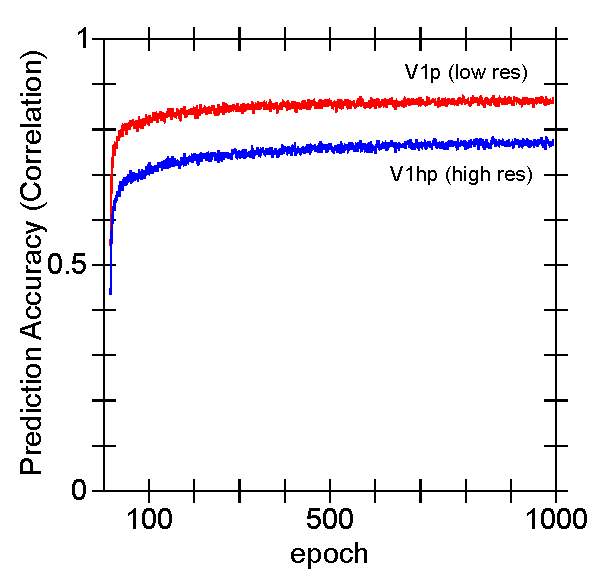
\includegraphics[width=2.5in]{figs/fig_deepleabra_wwi_emer_lrn_bp}
  \caption{Learning curves for the backpropagation version of the WWI model.  Although it achieves better predictive accuracy than the DeepLeabra version, it fails to acquire abstract object category structure, indicating a potential tradeoff between simplifying and categorizing inputs, versus predicting precisely where the low-level visual features will move.}
  \label{fig.bp_lrn}
\end{figure}

The backpropagation version of the WWI model has exactly the same layer sizes and {\em feedforward} patterns of connectivity as the DeepLeabra version.  Topographically, the V1p and V1hp pulvinar layers serve as output layers at the highest level of the network, receiving all the various connections from deep layers as shown in Table~\ref{tab.layer_sizes}.  Likewise, the LIPp served as a target output layer for the Where pathway.  To achieve predictive learning, the V1 pulvinar targets were from the scene at time $t$, while the V1s inputs were from the scene at time $t-1$.  We also ran a comparison auto-encoder model that had inputs and target outputs from the same time step, and it showed even less systematic organziation of its higher-level representations, further supporting the notion that predictive learning is important, across all frameworks.  The learning curve for the predictive version is shown in Figure~\ref{fig.bp_lrn}, which shows better overall prediction accuracy compared to the DeepLeabra model.  However, as the RSA showed, this backpropagation model failed to learn object categories that go beyond the input similarity structure, indicating that perhaps it was paying too much ``attention'' in learning to this low-level structure, and lacked the necessary mechanisms to enable it to impose a simplifying higher-level structure on top of these inputs.

\section{PredNet Model Methods}

The PredNet architecture was designed to incorporate principles from predictive coding theory into a neural network model for predicting the next frame in a video sequence. Details of the model can be found in the original paper %\cite{LotterKreimanCox16}
{\em (14)}, but here we provide a brief overview of the architecture. 

\subsection{Architecture}

PredNet is a deep convolutional neural network that is composed of layers containing discrete modules. The lowest layer generates a prediction of incoming inputs (i.e. the pixels in the next frame), while each of the higher layers attempts to predict the {\em errors} made by the previous layer. Each layer contains an input convolutional module ($A_l$), a recurrent representational module ($R_l$), a prediction module ($\hat{A}_l$), and a representation of its own errors ($E_l$). The input convolutional module ($A_l$) transforms its input with a set of standard convolutional filters, a rectified linear activation function, and a max-pooling operation. The recurrent representation module ($R_l$) is a convolutional LSTM, which is a recurrent convolutional network that replaces the matrix multiplications in the standard LSTM equations with convolutions, allowing it to maintain a spatially organized representation of its inputs over time. The prediction module ($\hat{A_l}$) consists of another standard convolutional layer and rectified linear activation that is used to generate predictions from the output of $R_l$. These predictions are then compared against the output of the input convolutional module ($A_l$). The errors generated in this comparison are represented explicitly in $E_l$, which applies a rectified linear activation to a concatenation of the positive ($A_l - \hat{A}_l$) and negative ($\hat{A}_l - A_l$) prediction errors. These errors then become the inputs to the next layer. 

\begin{equation}
A_l^t = 
\begin{cases}
    x_t, & \text{if } l = 0\\
    MaxPool(ReLU(Conv(E_{l-1}^t))), & \text{if } l > 0
\end{cases}
\end{equation}
\begin{equation}
\hat{A}_l^t = ReLU(Conv(R_l^t))
\end{equation}
\begin{equation}
E_l^t = [ReLU(A_l^t - \hat{A}_l^t); ReLU(\hat{A}_l^t - A_l^t)]
\end{equation}
\begin{equation}
R_l^t = ConvLSTM(E_l^{t-1},R_l^{t-1},UpSample(R_{l+1}^t))
\end{equation}

At each time step in the video sequence, PredNet generates a prediction of the next frame. This is done as follows: first, the $R_l$ is computed for each layer starting from the top of the hierarchy (because each $R_l^t$ depends on input from $R_{l+1}^t$), and then the $A_l^t$, $\hat{A}_l^{t}$ and $E_l^t$ are computed in a feed-forward fashion (becauase each $A_l^t$ depends on input from the layer below, $E_{l-1}^t$). 

% (JLR) Fixed $\hat{A}_l^{t+1}$ to be $\hat{A}_l^{t}$. This always confuses me. I had it right originally, then I changed it, but now it is correct.

All analyses in the RSA were conducted using the representations from the $R_l$ layers. 

\begin{figure}
  \centering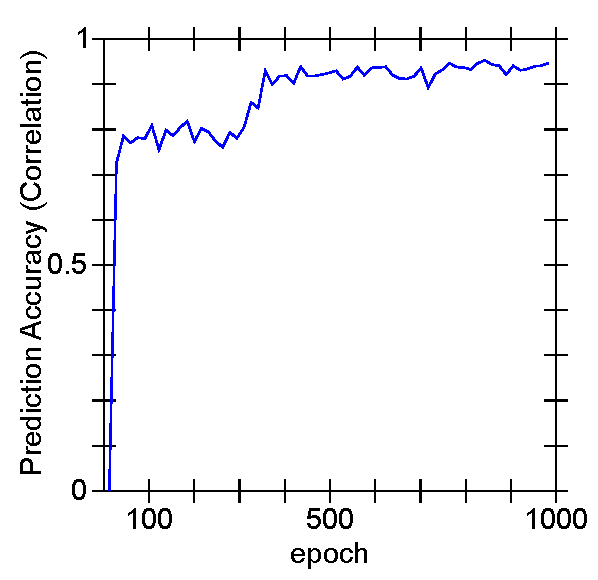
\includegraphics[width=2.5in]{figs/fig_deepleabra_wwi_emer_lrn_prednet}
  \caption{Learning curves for the PredNet model.  This model achieves the best overall prediction performance but also has the least well differentiated, categorical representations.}
  \label{fig.prednet_lrn}
\end{figure}

\subsection{Implementation details}

All experiments with the PredNet architecture were performed using PyTorch. An informal hyperparameter search was conducted, starting from the hyperparameters reported in the original paper. Our final architecture had 6 layers with 3, 16, 32, 64, 128, and 256 filters in the $A_l$ and $R_l$ modules, and 3x3 kernels throughout the whole network. However, we found that using sigmoid and tanh activation functions in fully-connected convolutional LSTMs slightly improved performance, so these were used for all experiments.

The weights in the PredNet model are trained using error backpropagation. Predictions are generated and errors are computed at all levels of the hierarchy, but the model performs better when only the lowest layer's errors are backpropagated %\cite{LotterKreimanCox16}
{\em (14)}. We confirmed these results with experiments that backpropagated the errors in higher layers, in which performance (in terms of mean squared error) was marginally reduced but the RSA results were similar. For this reason, all reported experiments used a PredNet that was trained by only backpropagating the lowest level error.

The model was trained using a batch size of 8 and an Adam optimizer with a learning rate of 0.0001, with no scheduler, for 150,000 batches.  A training curve is shown in Figure~\ref{fig.prednet_lrn}, showing that it achieves the best overall prediction accuracy of any model we tested, and yet has the least well differentiated, categorical representations, as shown in the main paper.

\subsection{Regularization experiments}

As discussed in the main paper, our biologically based model includes a number of important biologically motivated properties that may be contributing to the development of its categorical representations. These properties, including excitatory bidirectional connections, inhibitory competition, and an additional form of Hebbian learning, may be acting as regularizers that encourage categorical learning. We therefore tested whether standard regularization methods used in deep learning research would have similar effects on the representations developed in the PredNet architecture. We tested 1) batch normalization, 2) dropout, and 3) weight decay. 

% (JLR) y-axis on all of these training curves should say prediction accuracy - not prediction error
% (JLR) my initials are wrong in the "author contributions" section of the main paper
% (JLR) all references to PredNet "layer3" should now be layer 5 (or layer 6, depending on if you start counting from 0)



\end{document}
